\section{Pendahuluan}
Dalam fungsi URL yaitu untuk menampilkan sebuah website dalam website oracle apex, mungkin penjelasannya masih bingung, jadi seperti ini, dalam halaman oracle misalkan halaman TEST PAGE yang kita buat lalu kita akan membuat sebuah page di dalam halaman tersebut page tersebut berisikan halaman yang muncul dari URL lain, seperti halnya iFrame pada HTML.

\par IFRAME merupakan sebuah tag html yang berfungsi untuk menampilkan halaman website tanpa harus membuka halaman baru pada browser, pengguna akan disajikan halaman yang sudah ada seperti membuka website di dalam website.

\par Dalam penggunaan di oracle apex iframe dapat ditemukan pada tab Region yaitu URL yang dimana kita hanya memasukkan URL yang akan ditampilkan pada suatu halaman di oracle APEX tersebut.

\par Berikut adalah cara untuk membuat iFrame pada Oracle Apex:

\begin{enumerate}
\begin{figure}
    \item Pertama kita lihat pada tab regions lalu kita pilih URL, lihat pada Gambar 11.1.
        
        \centering
        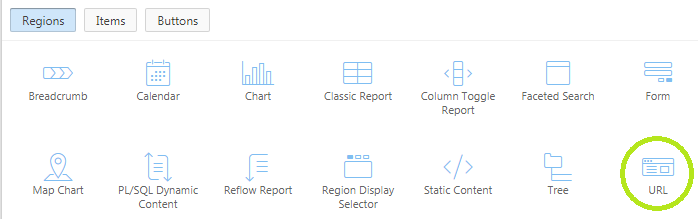
\includegraphics[scale=0.5]{figures/bab12/1.png}
        \caption{\textit{URL iFrame}}
        \label{URL iFrame}
    \end{figure}
    
    \begin{figure}
    \item Kemudian tarik dan lepaskan pada Content Body dibawah Test Page, lihat pada Gambar 11.2.
        
        \centering
        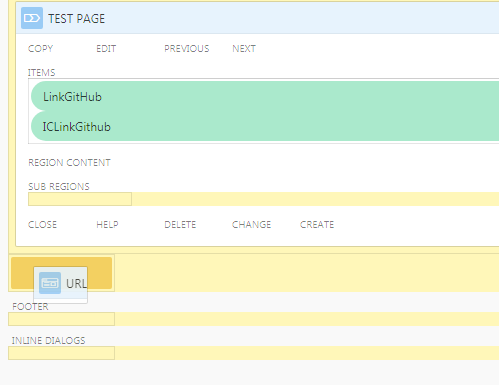
\includegraphics[scale=0.5]{figures/bab12/2.png}
        \caption{\textit{URL iFrame 2}}
        \label{URL iFrame 2}
    \end{figure}
    
    \begin{figure}
    \item Pada tab Identification kita beri Nama Title, lihat pada Gambar 11.3.
        
        \centering
        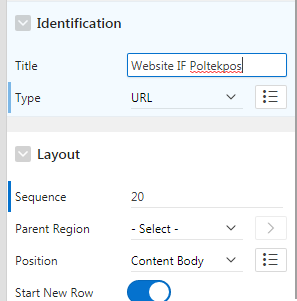
\includegraphics[scale=0.5]{figures/bab12/3.png}
        \caption{\textit{URL iFrame 3}}
        \label{URL iFrame 3}
    \end{figure}
    
    \begin{figure}
    \item Selanjutnya lihat pada menu navigasi di sebelah kiri klik Attributes yang sudah ditandai dengan warna merah dan bulatan hitam, lihat pada Gambar 11.4.
        
        \centering
        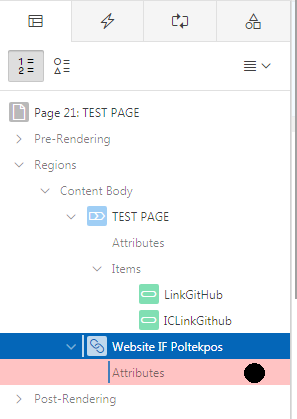
\includegraphics[scale=0.5]{figures/bab12/4.png}
        \caption{\textit{URL iFrame 4}}
        \label{URL iFrame 4}
    \end{figure}
    
    \begin{figure}
    \item Lalu masukkan URL salah satu website contoh \textit{https://if.poltekpos.ac.id} lalu masukan IFrame Attributes yaitu atribut dari iframe misalkan tinggi dan lebar IFrame yang diinginkan, lihat pada Gambar 11.5.
        
        \centering
        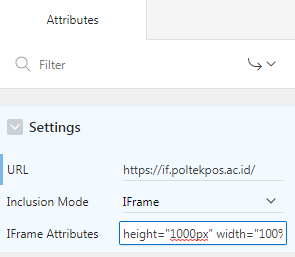
\includegraphics[scale=0.5]{figures/bab12/5.png}
        \caption{\textit{URL iFrame 5}}
        \label{URL iFrame 5}
    \end{figure}
    
    \begin{figure}
    \item Klik save dan bila sudah di Run akan menampilkan halaman seperti berikut, lihat pada Gambar 11.6.
        
        \centering
        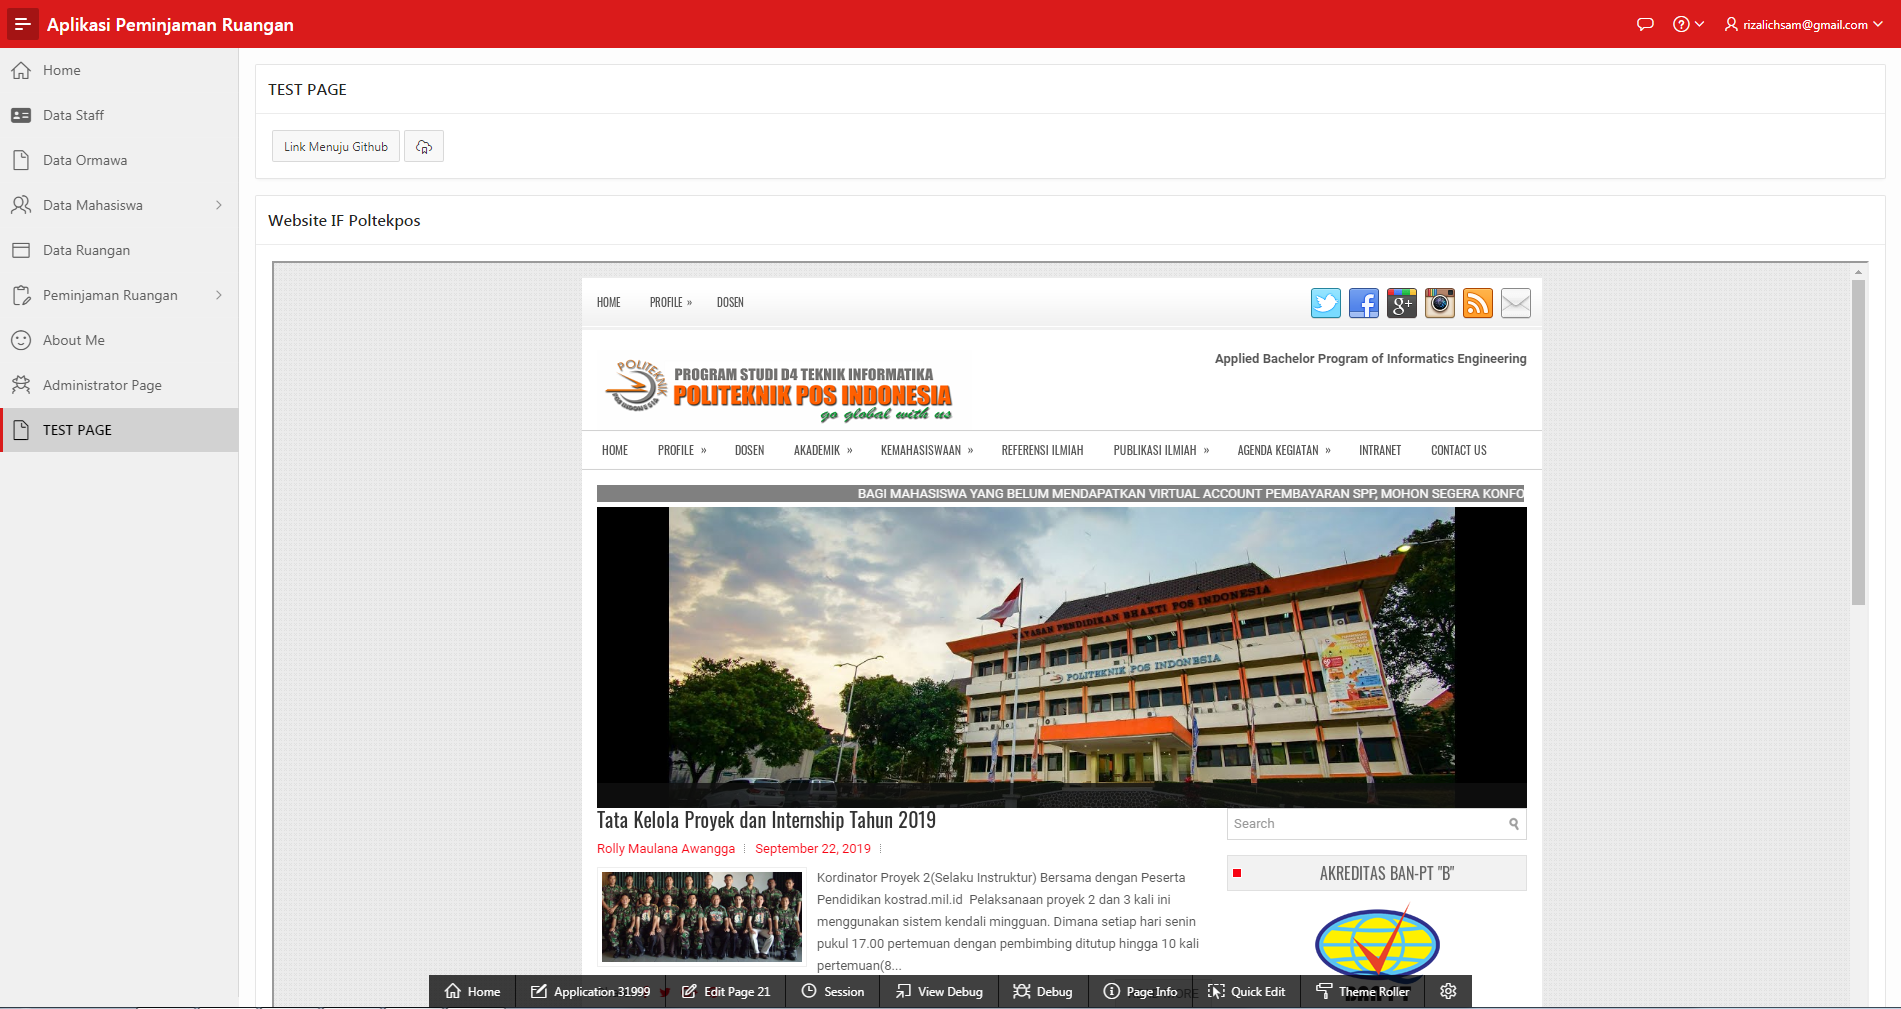
\includegraphics[scale=0.22]{figures/bab12/6.png}
        \caption{\textit{URL iFrame 6}}
        \label{URL iFrame 6}
    \end{figure}
    
    
\end{enumerate}
 